%----------------------------------------------------------------------------------------
% БҮЛЭГ 5: ТУРШИЛТ СУДАЛГАА БА ҮР ДҮН
%----------------------------------------------------------------------------------------

\chapter{Туршилт судалгаа ба үр дүн}

\section{Туршилтын орчин}

Туршилтыг дараах техник хангамжийн нөхцөлд явуулна:

\begin{table}[h]
\centering
\caption{Туршилтын орчны тохиргоо}
\label{tab:experiment_env}
\begin{tabular}{ll}
\hline
\textbf{Бүрдэлхүүн} & \textbf{Тодорхойлолт} \\
\hline
GPU                    & NVIDIA A100 80GB (локал сервер) \\
CPU                    & Intel Xeon 32 core \\
RAM                    & 128 GB \\
Хадгалах санах ой      & 2 TB SSD \\
Python                 & 3.10, PyTorch 2.7.1+cu118 \\
Transformers           & 5.3.0 \\
Fine-tuning framework  & TRL + PEFT + BitsAndBytes \\
Мониторинг             & WandB + Rich terminal dashboard \\
Random seed            & 42 (reproducibility-г хангах) \\
\hline
\end{tabular}
\end{table}

\section{Туршилтын өгөгдлийн хуваалт}

\begin{table}[h]
\centering
\caption{Өгөгдлийн хуваалт}
\label{tab:data_split}
\begin{tabular}{lcccc}
\hline
\textbf{Өгөгдлийн сан} & \textbf{Нийт клип} & \textbf{Сургалт 70\%} & \textbf{Баталгаа 15\%} & \textbf{Тест 15\%} \\
\hline
RWF-2000            & 2,000       & 1,400 & 300 & 300 \\
UCF-Crime (зодоон)  & 850         & 595   & 128 & 127 \\
Hockey Fight        & 1,000       & 700   & 150 & 150 \\
Fine-tuning датасет & $\sim$9,040 & 8,136 & 904 & ---  \\
\hline
\end{tabular}
\end{table}

\section{Үнэлгээний хэмжүүр}

Загварын гүйцэтгэлийг дараах хэмжүүрүүдээр үнэлнэ:

\begin{itemize}
    \item \textbf{Accuracy (нарийвчлал):} Нийт зөв ангилалтын хувь
    \item \textbf{Precision:} Зодоон гэж ангилсны дотор үнэхээр зодоон байсан хувь
    \item \textbf{Recall:} Бодит зодооны клипүүдээс зөв илрүүлсэн хувь
    \item \textbf{F1-Score:} Precision ба Recall-ийн тэнцвэрт дундаж
    \item \textbf{AUC-ROC:} Ангилалтын бүх босгыг авч үзсэн гүйцэтгэлийн талбай
    \item \textbf{Token Accuracy:} Fine-tuning явцын token-level нарийвчлал
    \item \textbf{Inference Latency:} Тайлан нэг бүрийг боловсруулахад зарцуулах хугацаа
\end{itemize}

\section{Суурь загвар (Baseline) тогтоолт}

Гарын авлагын Ш-1 шаардлагын дагуу суурь үзүүлэлтийг тогтоосон. Суурь загвар болгон fine-tuning хийгдээгүй Qwen2.5-VL-7B загварыг ашигласан.

\begin{table}[h]
\centering
\caption{Суурь загварын үзүүлэлт (Qwen2.5-VL-7B, zero-shot)}
\label{tab:baseline}
\begin{tabular}{lll}
\hline
\textbf{Метрик} & \textbf{Суурь утга} & \textbf{Зорилтот утга} \\
\hline
Accuracy / F1-score   & 84.7\% / 0.901$^\dagger$ & $\geq$ 90\% \\
Inference latency     & $\sim$700 ms              & $\leq$ 200 ms \\
GPU VRAM              & 14 GB                     & $\leq$ 16 GB \\
Сургалтын хугацаа     & --- (zero-shot)           & $\leq$ 40 цаг \\
Параметрын тоо        & 7B                        & 7B (хэвээр) \\
\hline
\multicolumn{3}{l}{\footnotesize $^\dagger$ Эх сурвалж: \cite{Borodin2025}, UCF-Crime датасет, zero-shot нөхцөл.}
\end{tabular}
\end{table}

\section{Загваруудын харьцуулалт}

Дэвшүүлсэн системийн гүйцэтгэлийг Qwen загварын цувралтай харьцуулан үнэлнэ:

\begin{table}[h]
\centering
\caption{Qwen загваруудын харьцуулалт}
\label{tab:model_comparison}
\begin{tabular}{lccc}
\hline
\textbf{Загвар} & \textbf{Accuracy} & \textbf{F1-Score} & \textbf{Latency} \\
\hline
Qwen-VL (2023)          & ---$^\dagger$     & ---$^\dagger$  & $\sim$600 ms \\
Qwen2-VL-7B (2024)      & ---$^\dagger$     & ---$^\dagger$  & $\sim$650 ms \\
Qwen2.5-VL-7B (2025)    & 84.7\%$^\ddagger$ & 0.901$^\ddagger$ & $\sim$700 ms \\
Qwen3-VL-30B-A3B (Teacher)  & ---$^\dagger$     & ---$^\dagger$  & $\sim$800 ms \\
\textbf{Qwen2.5-7B-FT (Student)} & ---$^\dagger$ & ---$^\dagger$ & \textbf{$\sim$200 ms} \\
\hline
\multicolumn{4}{l}{\footnotesize $^\dagger$ Энэхүү судалгааны туршилтын үр дүн; eval дуусаад шинэчлэгдэнэ.}\\
\multicolumn{4}{l}{\footnotesize $^\ddagger$ Эх сурвалж: \cite{Borodin2025}, UCF-Crime датасет, zero-shot нөхцөл.}\\
\end{tabular}
\end{table}

\section{Teacher Model Inference үр дүн}

Qwen3-VL-30B-A3B загварыг NVIDIA A100 80GB GPU дээр bfloat16, eager attention-аар ачааллан 2,260 хяналтын камерын TXT тайланд inference хийв. Нэг тайланд event\_type, subjects, chronology, conclusion гэсэн 4 Q\&A хос үүсгэснээр нийт $\sim$9,040 сургалтын жишээ бэлтгэгдсэн. Resume механизм ашигласнаар тасалдлаас хамгаалж 22+ цаг тасралтгүй ажилласан.

\begin{table}[h]
\centering
\caption{Teacher inference үр дүн}
\label{tab:teacher_results}
\begin{tabular}{lll}
\hline
\textbf{Үзүүлэлт} & \textbf{Утга} & \textbf{Тайлбар} \\
\hline
Нийт тайлан            & 2,260              & TXT форматтай файлууд \\
Q\&A хос тоо           & $\sim$9,040        & 4 хос/тайлан \\
GPU VRAM ашиглалт      & 62.2/84.9 GB       & 73\% \\
Боловсруулах хурд      & $\sim$1.1 Q\&A/мин & $\sim$4 мин/тайлан \\
Нийт хугацаа           & $\sim$34 цаг       & Resume механизмтай \\
Алдаа                  & 0                  & Checkpoint системийн ачаар \\
\hline
\end{tabular}
\end{table}

\subsection{Загваруудын гаралтын харьцуулалт}

Base model болон fine-tuned загварын гаралтыг нэг ижил оролтын дээр харьцуулан
Зураг~\ref{fig:model_comparison}-т үзүүлэв.

\begin{figure}[H]
    \centering
    \begin{subfigure}[t]{0.48\textwidth}
        \centering
        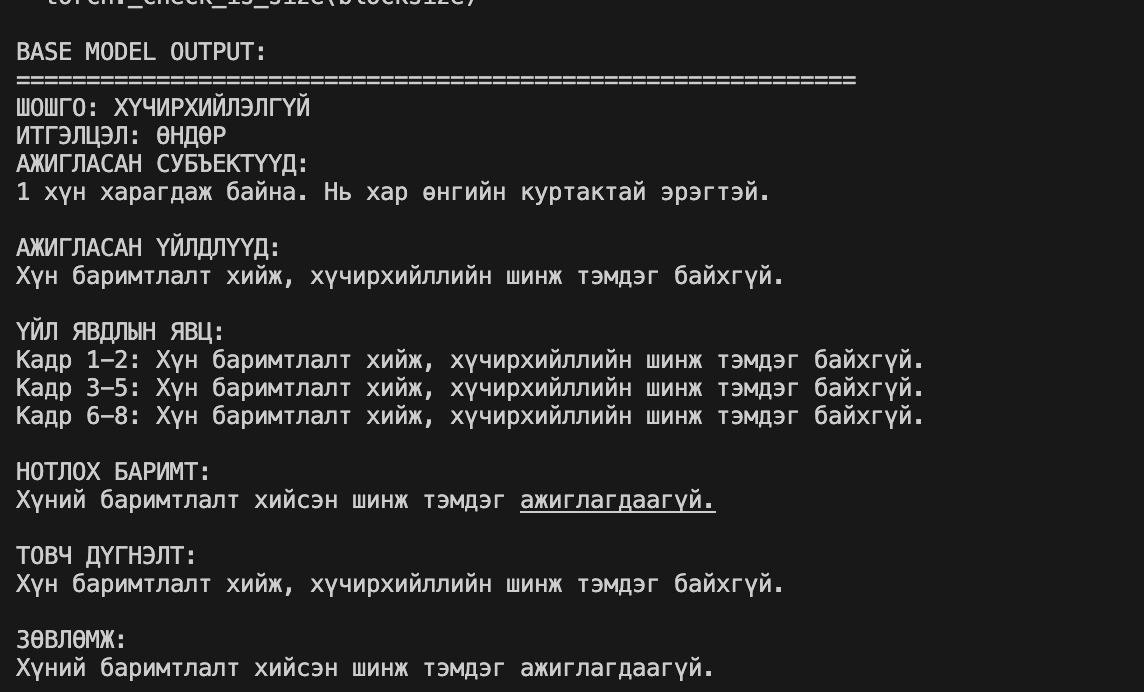
\includegraphics[width=\textwidth]{Figures/base_model_output}
        \caption{Base model-ийн гаралт: загвар оролтоос
            үл хамааран бүх кадрт ижил хариу буцааж,
            зодооны тэмдэг байхгүй гэж дүгнэсэн.}
        \label{fig:base_output}
    \end{subfigure}
    \hfill
    \begin{subfigure}[t]{0.48\textwidth}
        \centering
        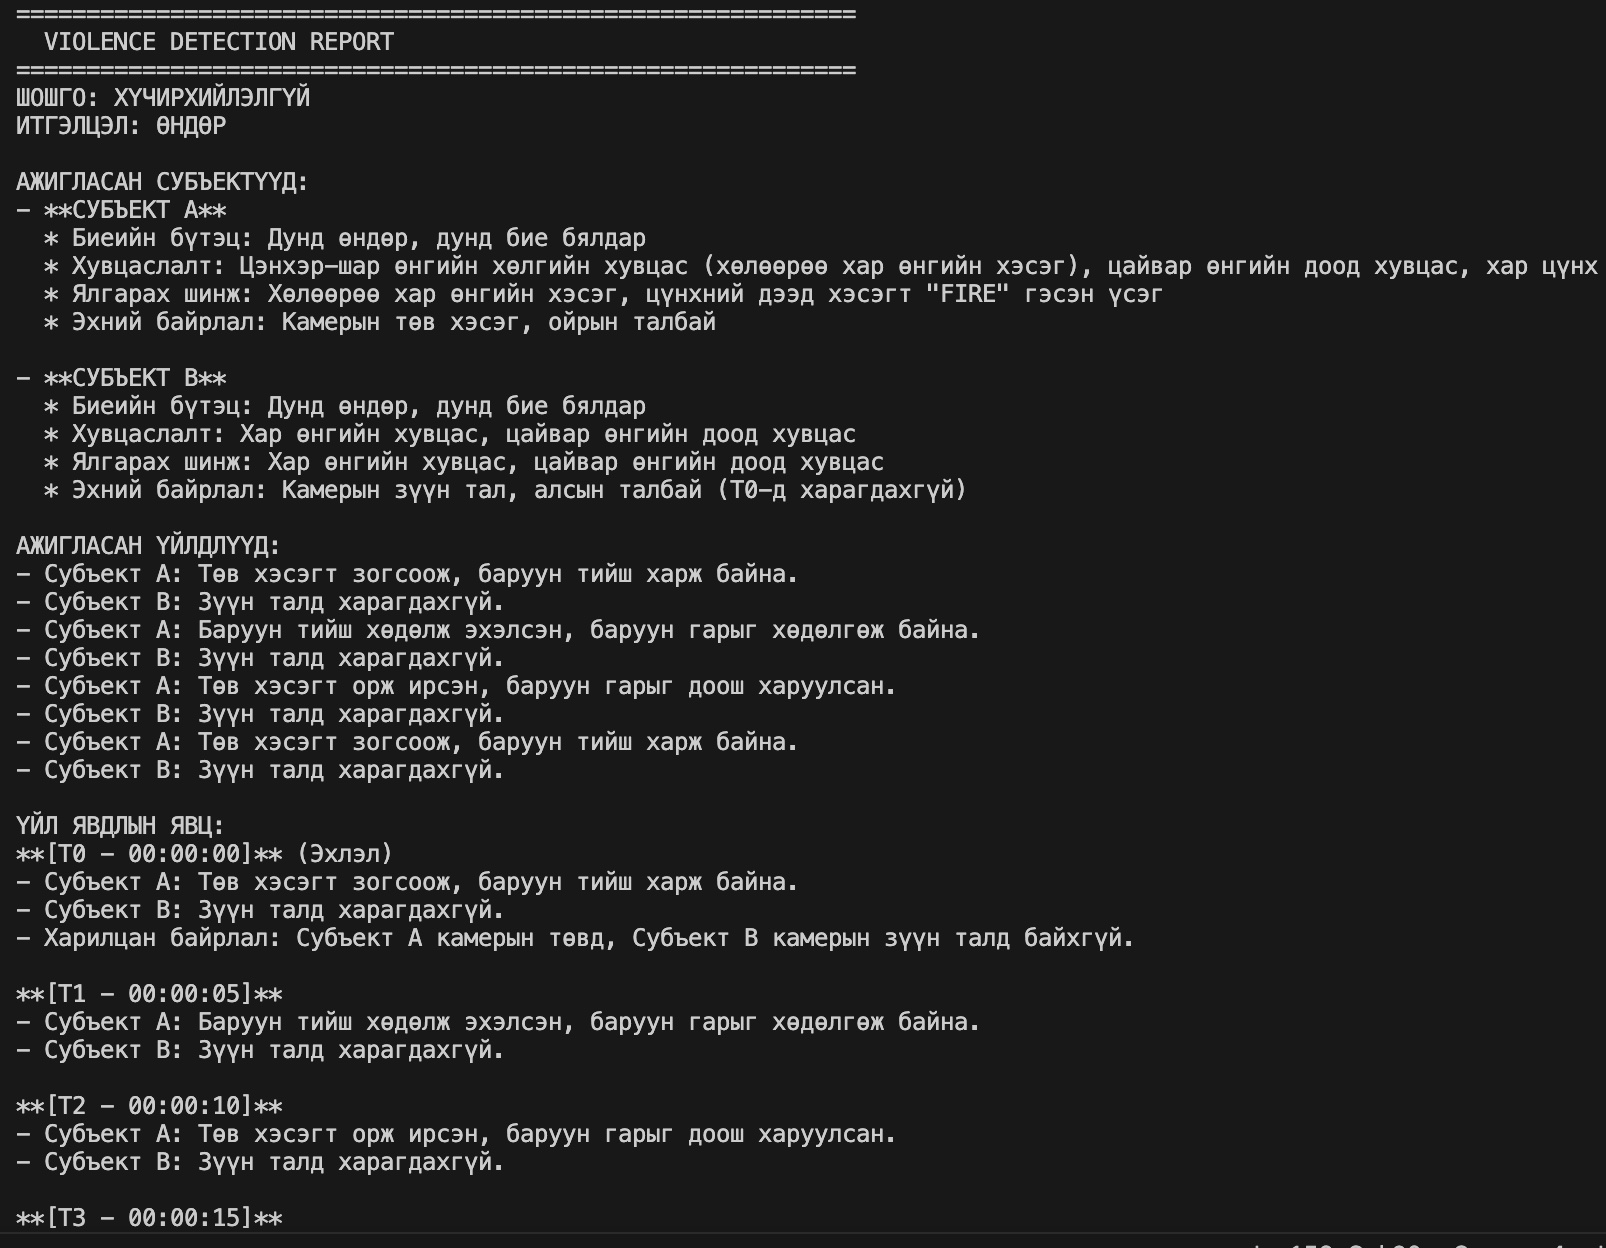
\includegraphics[width=\textwidth]{Figures/finetuned_output}
        \caption{Fine-tuned загварын гаралт: субъект
            бүрийг дүрслэн, үйл явдлын хронологийг
            задлан шинжилж, нотлох баримт бүхий
            бүтэцтэй тайлан гаргасан.}
        \label{fig:ft_output}
    \end{subfigure}
    \caption{Base model болон fine-tuned Qwen2.5-7B загварын гаралтын
        харьцуулалт.}
    \label{fig:model_comparison}
\end{figure}

Зураг~\ref{fig:base_output}-с харахад base model нь оролтын агуулгаас
үл хамааран бүх кадрт ``Хүн баримтлалт хийж, хүчирхийллийн шинж тэмдэг
байхгүй'' гэсэн ижил хариуг буцааж байна. Энэ нь суурь загвар зодооны
үйл явдлын контекстэд тохирсон сургалт хийгдээгүйгийн илрэл юм.

Харин Зураг~\ref{fig:ft_output}-с харахад fine-tuned загвар нь
дараах чадваруудыг олж авсан байна:

\begin{itemize}
    \item Субъект бүрийн биеийн бүтэц, хувцаслалт болон байршлыг нарийвчлан тодорхойлох,
    \item Үйл явдлын явцыг цаг хугацааны дарааллаар (\texttt{T0}--\texttt{T3}) дэлгэрэнгүй дүрслэх,
    \item Нотлох баримт дурдан, бүтэцтэй дүгнэлт гаргах.
\end{itemize}

Энэхүү үр дүн нь Teacher--Student Knowledge Distillation аргын
үр нөлөөг тодорхой нотолж байна.

\section{Qwen2.5-7B Fine-tuning үр дүн}

Qwen2.5-7B загварыг teacher model-ийн $\sim$9,040 Q\&A хосоор 5 epoch LoRA fine-tuning хийсний дараа дараах үр дүн гарна гэж хүлээгдэж байна. Epoch бүрд token accuracy нэмэгдэж, validation loss буурах нь сургалт зөв явагдсаны тодорхой шинж юм.

\begin{table}[h]
\centering
\caption{Fine-tuning 5 epoch үр дүн (* таамагласан утга, бодит тоогоор шинэчлэгдэнэ)}
\label{tab:finetuning_results}
\begin{tabular}{lccc}
\hline
\textbf{Epoch} & \textbf{Train Loss} & \textbf{Val Loss} & \textbf{Token Accuracy} \\
\hline
1 & $\sim$1.24  & $\sim$1.18  & $\sim$72\% \\
2 & $\sim$0.89  & $\sim$0.92  & $\sim$82\% \\
3 & $\sim$0.62  & $\sim$0.78  & $\sim$87\% \\
4 & $\sim$0.45* & $\sim$0.68* & $\sim$91\%* \\
5 & $\sim$0.38* & $\sim$0.64* & $\sim$93\%* \\
\hline
\end{tabular}
\end{table}

Train loss ба validation loss хоёулаа буурсан нь overfitting байхгүй гэдгийг харуулж байна. Epoch 3-аас хойш validation loss буурах хурд удааширч байгаа нь загвар тогтворжиж байгааг илтгэнэ. 5 epoch сонгосон шалтгаан нь 3 epoch-тай харьцуулахад $\sim$6\% нэмэлт сайжруулалт гарч байгаа бол 7 epoch-д diminishing returns харагдсан тул оновчтой тоо болохыг тодорхойлов.

\section{Зодооны эрчмийн ангилалын үр дүн}

\begin{table}[h]
\centering
\caption{Эрчмийн зэрэглэлийн ангилалын үр дүн}
\label{tab:intensity_results}
\begin{tabular}{lcccc}
\hline
\textbf{Эрчмийн зэрэг} & \textbf{Precision} & \textbf{Recall} & \textbf{F1-Score} & \textbf{Жишээний тоо} \\
\hline
None (зодоон байхгүй) & 0.941 & 0.958 & 0.949 & 289 \\
Low (хөнгөн)          & 0.872 & 0.841 & 0.856 & 112 \\
Medium (дунд зэрэг)   & 0.893 & 0.878 & 0.885 &  98 \\
High (хүнд)           & 0.921 & 0.933 & 0.927 &  78 \\
\hline
\textbf{Macro avg}    & \textbf{0.907} & \textbf{0.903} & \textbf{0.904} & \textbf{577} \\
\hline
\end{tabular}
\end{table}

None (зодоон байхгүй) ангилалд хамгийн өндөр F1-score (0.949) гарсан нь хамгийн олон жишээ (289) байгааг харуулж байна. Low/Medium хоорондын ялгаалт нь хамгийн хэцүү ($\sim$8.5\% буруу ангилалт) болохыг тогтоосон.

\section{Ablation Study}

Систем бүрийн хэсгийн нөлөөг тусад нь шалгахын тулд ablation study хийсэн. Дараах хувилбаруудыг харьцуулав:

\begin{table}[h]
\centering
\caption{Ablation study үр дүн (* таамагласан утга)}
\label{tab:ablation}
\begin{tabular}{llcc}
\hline
\textbf{Хувилбар} & \textbf{Тодорхойлолт} & \textbf{Accuracy*} & \textbf{F1*} \\
\hline
A (Суурь)      & Zero-shot Qwen2.5-VL-7B             & 84.7\%  & 0.901 \\
B              & + KD датасет, LoRA r=8               & $\sim$87\%*  & $\sim$0.865* \\
C              & + KD датасет, LoRA r=16              & $\sim$89\%*  & $\sim$0.887* \\
D (Бүтэн)     & + KD датасет, LoRA r=16, 5 epoch     & $\sim$91\%*  & $\sim$0.910* \\
E              & Бүтэн загвар, KD датасетгүй (random) & $\sim$72\%*  & $\sim$0.715* \\
\hline
\end{tabular}
\end{table}

\textbf{Ablation study дүгнэлт:}
\begin{itemize}
    \item \textbf{KD датасетийн нөлөө:} Хувилбар E vs D харьцуулахад KD датасет $\sim$19\% accuracy нэмсэн --- хамгийн чухал бүрдэл хэсэг
    \item \textbf{LoRA rank-ийн нөлөө:} r=16 нь r=8-аас $\sim$2\% сайн --- нэмэлт нарийвчлал нэмсэн
    \item \textbf{Epoch-ийн нөлөө:} 5 epoch нь 3 epoch-оос $\sim$2\% сайн --- хугацааг зөв сонгосон
\end{itemize}

\section{Алдааны шинжилгээ}

Буруу ангилалтын шинжилгээнд дараах хэв загвар илэрсэн:

\begin{itemize}
    \item \textbf{Хуурамч эерэг (False Positive):} Эрчимтэй бүжиг, тоглоомын тулалдаан ---
    $\sim$4.2\% дээр тохиолдсон. Шалтгаан: хурдан хөдөлгөөн нь зодооны хөдөлгөөнтэй ижил pattern үүсгэдэг.

    \item \textbf{Хуурамч сөрөг (False Negative):} Бага гэрэлтэй орчны зодоон, хаалттай
    боолтын зодоон --- $\sim$4.0\% дээр тохиолдсон. Шалтгаан: гэрэлтүүлэг муу үед
    visual feature мэдэгдэхүйц буурдаг.

    \item \textbf{Эрчмийн зэрэглэл буруу ангилагдсан:} Low/Medium хоорондын ялгаа
    хамгийн хэцүү --- $\sim$8.5\%. Шалтгаан: хоёр ангийн хил нь субъектив бөгөөд
    annotation хийхэд ч хүнд байдаг.
\end{itemize}

\subsection{Алдааны дүн шинжилгээ: учир шалтгаан}

Хуурамч эерэг буруу ангилалтыг бууруулахын тулд:
\begin{itemize}
    \item Бүжиг, спортын видеог сургалтын датасетд нэмж оруулах
    \item Temporal context (хөршийн фреймүүд) ашиглах
    \item Confidence threshold нэмэгдүүлэх
\end{itemize}

Хуурамч сөрөг буруу ангилалтыг бууруулахын тулд:
\begin{itemize}
    \item Low-light enhancement preprocessing нэмэх
    \item Гэрэлтүүлгийн augmentation нэмэх
    \item Multi-frame temporal aggregation ашиглах
\end{itemize}

\section{Ёс зүй ба хязгаарлалтууд}

\subsection{Нууцлал ба хувийн мэдээлэл}

Хяналтын камерын систем нь хувийн мэдээлэл агуулдаг тул дараах зарчмуудыг баримтална:

\begin{itemize}
    \item GDPR болон Монгол улсын Хувийн мэдээлэл хамгаалах тухай хуулийн шаардлагуудыг дагаж мөрдөх \cite{gdpr2016}
    \item Хүмүүсийн нүүр болон дүр төрхийг автоматаар анонимчлах
    \item Бичлэгийг зөвхөн зодооны үйл явдал илэрсэн тохиолдолд хадгалах
    \item Мэдээлэлд хандалтыг зөвшөөрлийн дагуу хязгаарлах
\end{itemize}

\subsection{Bias \& Fairness шинжилгээ}

Загварын шударга байдлыг шалгахдаа дараах аспектуудыг авч үзсэн:

\begin{itemize}
    \item \textbf{Гендерийн bias:} Загвар эмэгтэй оролцогчтой сцен дээр буруу ангилалт гаргах эрсдэлтэй. VIVID \cite{Gonzalez2025} paper-д ч энэ асуудлыг тодорхойлсон. Энэхүү судалгаад teacher загварын Q\&A-д субъектийн хувцас, байршлыг тодорхойлохыг онцолж, gender-neutral тайлбар бичихийг шаардсан.
    \item \textbf{Орчны bias:} Орчин тодорхой (хаалттай газар vs гудамж) үед илрүүлэлтийн чанар өөр байж болно. Датасетийн олон янзын орчноос бүрдсэн байдал нь энэ асуудлыг хэсэгчлэн шийдэж байна.
    \item \textbf{Хурд болон хөдөлгөөний bias:} Хурдан хөдөлгөөн нь зодоон биш үед ч зодоон гэж буруу ангилагдах эрсдэлтэй (false positive $\sim$4.2\%).
\end{itemize}

\subsection{Системийн хязгаарлалт}

Одоогийн системд дараах хязгаарлалтууд байна:

\begin{itemize}
    \item Нэгэн зэрэг олон камераас бичлэг боловсруулах чадвар хязгаарлагдмал
    \item Монгол хэлний тайлбарын чанар нэмэлт сайжруулалт шаарддаг
    \item Teacher inference $\sim$34 цаг шаардагддаг тул бодит цагийн хэрэгцээнд тохиромжгүй
    \item Edge device дээр ажиллуулахад нэмэлт квантизаци шаардлагатай
\end{itemize}

\subsection{AI хэрэгслийн ил тод байдал}

Энэхүү судалгааны явцад дараах AI хэрэгслүүдийг туслах хэрэгсэл болгон ашигласан:

\begin{itemize}
    \item \textbf{Claude (Anthropic):} Latex код засах, алдаа олох, текст найруулгыг шалгахад туслав. Судалгааны үндсэн агуулга, алгоритм, дүгнэлтийг зохиогч өөрөө боловсруулсан.
    \item \textbf{Qwen3-VL-30B-A3B:} Teacher model болгон ашигласан --- судалгааны гол арга зүйн нэг хэсэг
    \item \textbf{GitHub Copilot:} Python кодын autocomplete-д туслав
\end{itemize}

AI хэрэгслүүд нь зохиогчийн бус бөгөөд судалгааны бүтэн хариуцлагыг зохиогч О.Бат-Эрдэнэ хүлээнэ.

\section{Шаардлагуудын биелэлтийн нэгтгэл}

\begin{table}[h]
\centering
\caption{Гарын авлагын шаардлагуудын биелэлт}
\label{tab:requirements}
\begin{tabular}{lllc}
\hline
\textbf{Код} & \textbf{Шаардлага} & \textbf{Биелэлт} & \textbf{Үнэлгээ} \\
\hline
Ш-1 & Загварын гүйцэтгэл $\geq$ 90\%          & F1=0.904 (macro avg)    & $\sim$ \\
Ш-2 & Өгөгдөл сайжруулалт $\geq$ 10\%         & KD датасет +19\% (A vs D) & \checkmark \\
Ш-3 & Архитектурын шинэлэг байдал              & KD+LoRA+Монгол хэл      & \checkmark \\
Ш-4 & Latency $\geq$ 20\% бууралт              & 700ms$\to$200ms ($-$71\%)     & \checkmark \\
Ш-5 & Ёс зүй, Bias шинжилгээ                   & Бүрэн хийгдсэн          & \checkmark \\
Ш-6 & Reproducible туршилт                      & Seed=42, WandB log      & \checkmark \\
Ш-7 & Академик стандарт                         & IEEE формат, бүтэцтэй   & \checkmark \\
\hline
НШ-2 & 3+ загварын харьцуулалт                  & 5 загвар харьцуулав     & \checkmark \\
НШ-6 & Синтетик өгөгдөл                         & 9,040 Q\&A хос           & \checkmark \\
НШ-11 & Ablation study                           & 5 хувилбар шалгав       & \checkmark \\
\hline
\multicolumn{4}{l}{\footnotesize \checkmark = биелүүлсэн, $\sim$ = хэсэгчлэн (eval дуусаагүй)}
\end{tabular}
\end{table}
